\documentclass[12pt]{article}

% TEMPLATE DEFAULT PACKAGES
\usepackage{amssymb,amsmath,amsfonts,eurosym,geometry,ulem,graphicx,caption,color,setspace,sectsty,comment,footmisc,caption,natbib,pdflscape,array,hyperref,adjustbox}

% ADDED PACKAGES FOR THIS MANUSCRIPT
\usepackage{mathptmx,multirow,titlesec,threeparttable,tabu,booktabs,titlesec,subfigure,threeparttable,mathtools,bm,bbm}
% endfloat,
\usepackage{rotating}

% SECTION TITLE SETTINGS
\titlelabel{\thetitle.\enskip}
\titleformat*{\section}{\large\bfseries}
\titleformat*{\subsection}{\normalsize\bfseries}

% COLUMN TYPES
\newcolumntype{L}[1]{>{\raggedright\let\newline\\\arraybackslash\hspace{0pt}}m{#1}}
\newcolumntype{C}[1]{>{\centering\let\newline\\\arraybackslash\hspace{0pt}}m{#1}}
\newcolumntype{R}[1]{>{\raggedleft\let\newline\\\arraybackslash\hspace{0pt}}m{#1}}

% MARGINS AND SPACING
\normalem
%\onehalfspacing
\geometry{left=1in,right=1in,top=1.0in,bottom=1.0in}

% SPECIAL CELL 
\newcommand{\specialcell}[2][c]{%
	\begin{tabular}[#1]{@{}l@{}}#2\end{tabular}}

\begin{document}{}

\section{Set Up}
Let there be discrete locations $j$ be located on a horizontal line from $1$ to $J$, each with a formal, $F$, and informal, $I$, housing market.  

Let there be $N$ total homogeneous households where each household $i$ needs to choose where to live and whether to rent from the formal, $F$, or informal, $I$, housing sectors.  Housing supply in location $j$ and sector $s$ is given by $r_{j,s}=z_{j,s}+k_s N_{j,s}$ where $N_{j,s}$ measures the number of people choosing this location and sector.


Utilities for household $i$ choosing formal or informal housing in location $j$ are given by:
\begin{align*}
u_{i,F}   &= - z_{j,F}  - k_F N_{j,F}  - \lambda N_{j,I} - \gamma (N_{j-1,I}+N_{j+1,I})  \\
u_{i,I}   &= - z_{j,I}  - k_I N_{j,I}  - \lambda N_{j,I} - \gamma (N_{j-1,I}+N_{j+1,I}) 
\end{align*}
$\lambda$ is a reduced-form way of capturing any negative externalities caused by local informal housing in location $j$.  Likewise, $\gamma$ captures any negative externalities caused by informal housing in neighboring areas $j-1$ and $j+1$.

Spatial equilibrium in this framework is reached when households move across locations and housing sectors so that utilities across all sectors are equalized.

\section{Bring to Data}
The next exercise uses this model to recreate observed building densities.  Here are the simulation values (at baseline):
\begin{align*}
J &= 4 \\
z_{1,I} &= 0.5 \\
z_{1,F} &= 2 \\
z_{-1,I} &= z_{-1,F} = 1 \\
k_{F} = k_{I} &= 1  \\
\lambda &= .5 \\
\gamma &= .4
\end{align*}

Moving from 2001 to 2011, total population increases from $N=20$ to $N=25$.  All other parameters stay the same for unconstructed projects.  For constructed projects, moving from 2001 to 2011 reduces the fixed costs for formal houses $z_{1,F}$ from 2 to 1.2 and increases the fixed costs for informal houses $z_{1,I}$ from .5 to 0.8, which is how this model captures the construction of housing projects.

\section{Analysis}

The first thing to notices looking at all the figures (but especially Figure~\ref{fig3}) is the hump shape of the distribution.  Focusing on Figure~\ref{fig3}, low construction costs for informal housing in the project area (at x-axis=1) mean that we get a large density of informal housing.  Since these informal houses produce negative amenities, the neighboring area (at 2) builds less informal housing.  This reduction in informal housing (at 2) a second order effect of increasing the desirability of living just further away (at 3).  Finally this increase in informal housing makes it less desirable to live furthest from the project (at 4).


\begin{figure}[b]
\caption{Formal Unconstructed}\label{fig1}
\centering
\begin{minipage}[b]{.4\textwidth}
\centering
%\hspace{1cm}Theory
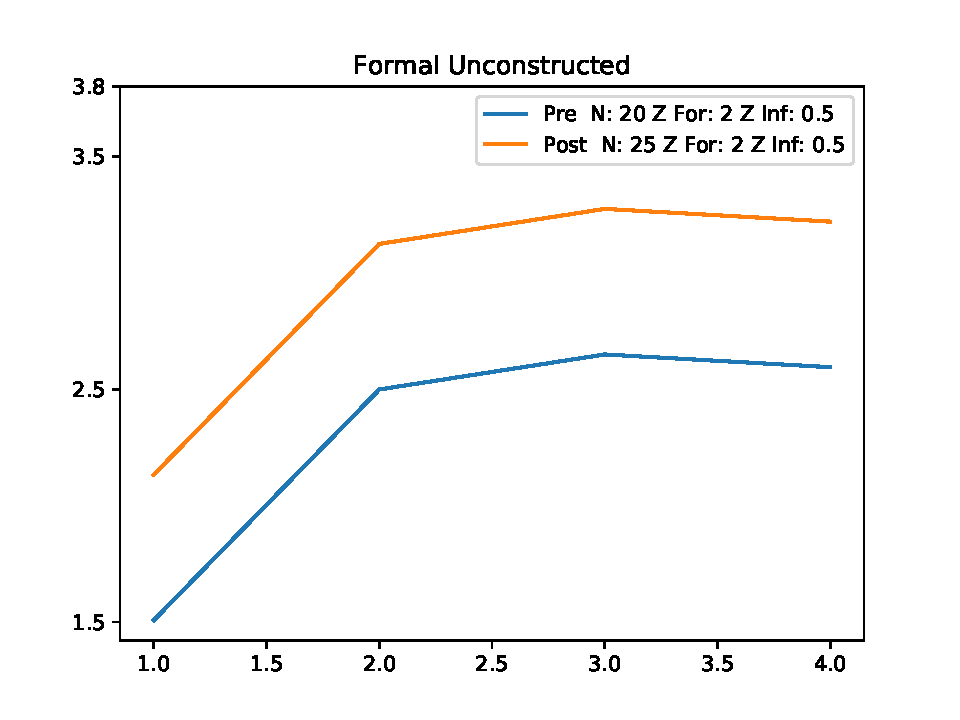
\includegraphics[scale=.48]{figures/unconstructed_formal.pdf}
\end{minipage}
\begin{minipage}[b]{.4\textwidth}
\centering
%\hspace{1cm}Data
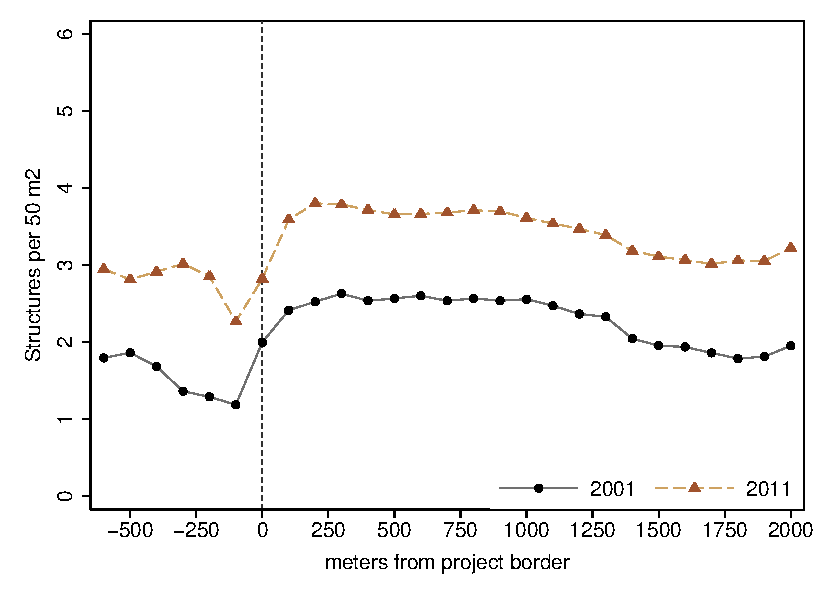
\includegraphics[scale=.5]{figures/bblu_for_placebo_admin.pdf}
\end{minipage}
\end{figure}


\begin{figure}[b]
\caption{Formal Constructed}\label{fig2}
\centering
\begin{minipage}[b]{.4\textwidth}
\centering
%\hspace{1cm}Theory
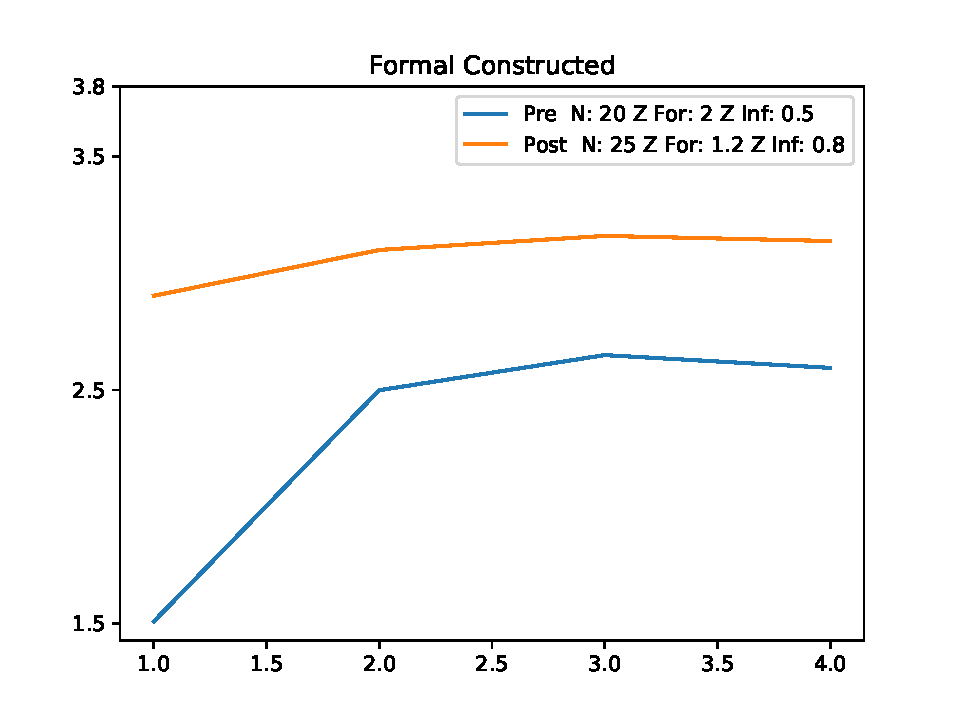
\includegraphics[scale=.48]{figures/constructed_formal.pdf}
\end{minipage}
\begin{minipage}[b]{.4\textwidth}
\centering
%\hspace{1cm}Data
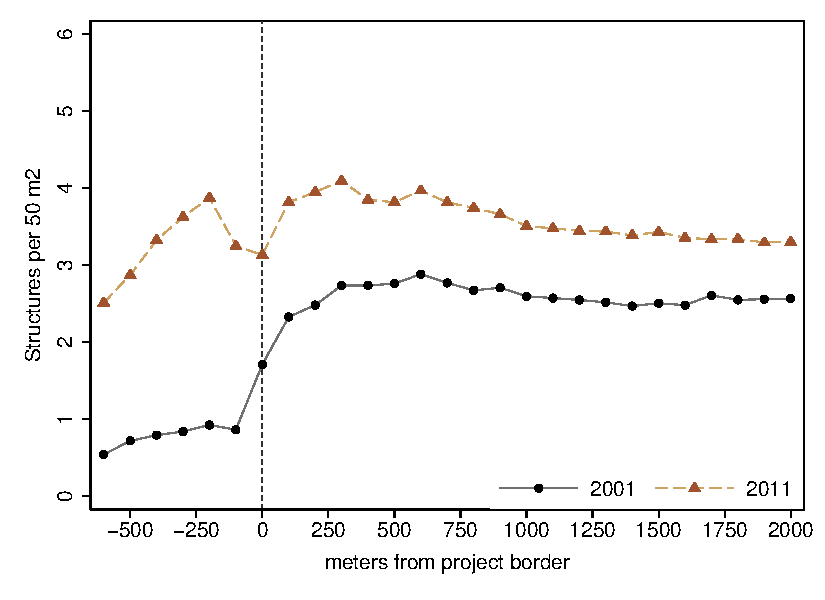
\includegraphics[scale=.5]{figures/bblu_for_rdp_admin.pdf}
\end{minipage}
\end{figure}



\begin{figure}[b]
\caption{Informal Unconstructed}\label{fig3}
\centering
\begin{minipage}[b]{.4\textwidth}
\centering
%\hspace{1cm}Theory
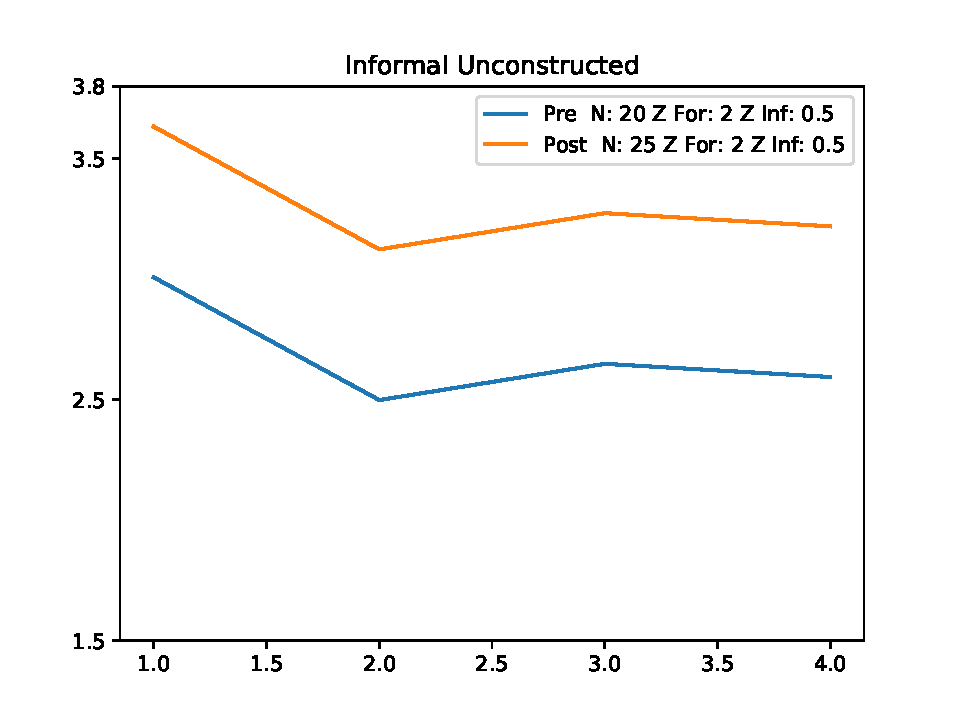
\includegraphics[scale=.48]{figures/unconstructed_informal.pdf}
\end{minipage}
\begin{minipage}[b]{.4\textwidth}
\centering
%\hspace{1cm}Data
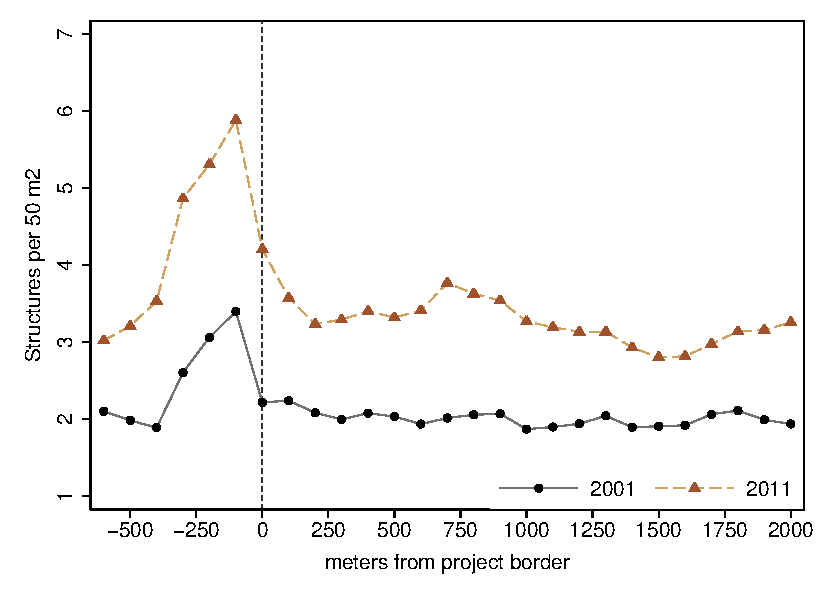
\includegraphics[scale=.5]{figures/bblu_inf_placebo_admin.pdf}
\end{minipage}
\end{figure}


\begin{figure}[b]
\caption{Informal Constructed}\label{fig4}
\centering
\begin{minipage}[b]{.4\textwidth}
\centering
%\hspace{1cm}Theory
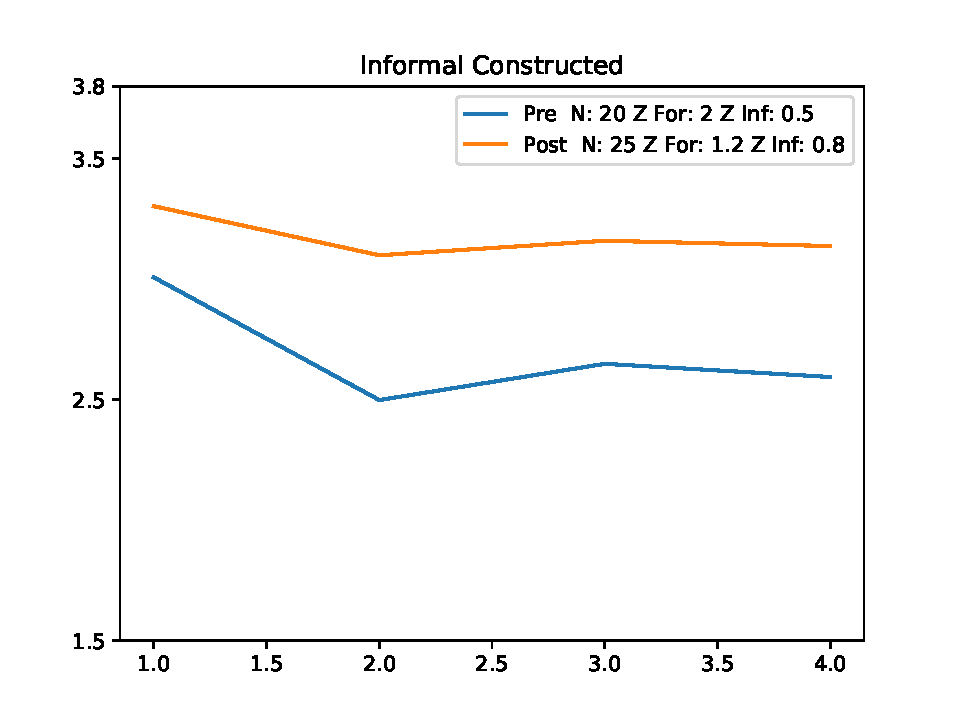
\includegraphics[scale=.48]{figures/constructed_informal.pdf}
\end{minipage}
\begin{minipage}[b]{.4\textwidth}
\centering
%\hspace{1cm}Data
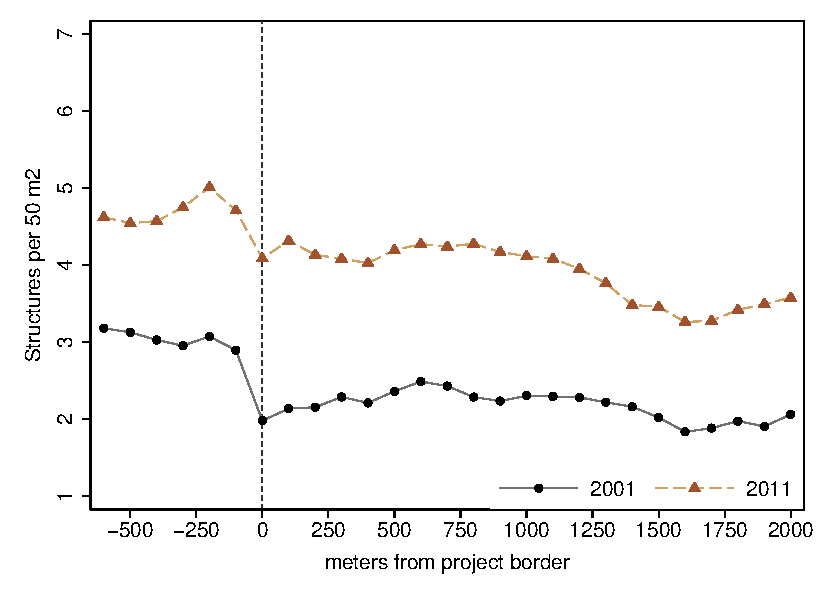
\includegraphics[scale=.5]{figures/bblu_inf_rdp_admin.pdf}
\end{minipage}
\end{figure}


\pagebreak

\begin{align*}
\frac{2 N g^{3} k ki - N g^{2} gd k ki - N g^{2} k ki^{2} - 2 N g gd^{2} k ki - 4 N g gd k ki^{2} - 2 N g k ki^{3} + N gd^{3} k ki + 3 N gd^{2} k ki^{2} + 3 N gd k ki^{3} + N k ki^{4} - 8 g^{3} k z_{1} + 8 g^{3} k z1i - 6 g^{3} ki z_{1} + 6 g^{3} ki z1i + 2 g^{3} ki z_{2} - 2 g^{3} ki z2i + 2 g^{3} ki z_{3} - 2 g^{3} ki z3i + 2 g^{3} ki z_{4} - 2 g^{3} ki z4i + 4 g^{2} gd k z_{1} - 4 g^{2} gd k z1i + 3 g^{2} gd ki z_{1} - 3 g^{2} gd ki z1i - g^{2} gd ki z_{2} + g^{2} gd ki z2i - g^{2} gd ki z_{3} + g^{2} gd ki z3i - g^{2} gd ki z_{4} + g^{2} gd ki z4i + 4 g^{2} k ki z_{1} - 4 g^{2} k ki z1i - 6 g^{2} k ki z2i + 2 g^{2} k ki z3i + 4 g^{2} k ki z4i + 3 g^{2} ki^{2} z_{1} - 3 g^{2} ki^{2} z1i - g^{2} ki^{2} z_{2} - 5 g^{2} ki^{2} z2i - g^{2} ki^{2} z_{3} + 3 g^{2} ki^{2} z3i - g^{2} ki^{2} z_{4} + 5 g^{2} ki^{2} z4i + 8 g gd^{2} k z_{1} - 8 g gd^{2} k z1i + 6 g gd^{2} ki z_{1} - 6 g gd^{2} ki z1i - 2 g gd^{2} ki z_{2} + 2 g gd^{2} ki z2i - 2 g gd^{2} ki z_{3} + 2 g gd^{2} ki z3i - 2 g gd^{2} ki z_{4} + 2 g gd^{2} ki z4i + 16 g gd k ki z_{1} - 11 g gd k ki z1i + 3 g gd k ki z2i - 5 g gd k ki z3i - 3 g gd k ki z4i + 12 g gd ki^{2} z_{1} - 7 g gd ki^{2} z1i - 4 g gd ki^{2} z_{2} + 7 g gd ki^{2} z2i - 4 g gd ki^{2} z_{3} - g gd ki^{2} z3i - 4 g gd ki^{2} z_{4} + g gd ki^{2} z4i + 8 g k ki^{2} z_{1} - 3 g k ki^{2} z1i + 3 g k ki^{2} z2i - 5 g k ki^{2} z3i - 3 g k ki^{2} z4i + 6 g ki^{3} z_{1} - g ki^{3} z1i - 2 g ki^{3} z_{2} + 5 g ki^{3} z2i - 2 g ki^{3} z_{3} - 3 g ki^{3} z3i - 2 g ki^{3} z_{4} - g ki^{3} z4i - 4 gd^{3} k z_{1} + 4 gd^{3} k z1i - 3 gd^{3} ki z_{1} + 3 gd^{3} ki z1i + gd^{3} ki z_{2} - gd^{3} ki z2i + gd^{3} ki z_{3} - gd^{3} ki z3i + gd^{3} ki z_{4} - gd^{3} ki z4i - 12 gd^{2} k ki z_{1} + 9 gd^{2} k ki z1i + gd^{2} k ki z2i + gd^{2} k ki z3i + gd^{2} k ki z4i - 9 gd^{2} ki^{2} z_{1} + 6 gd^{2} ki^{2} z1i + 3 gd^{2} ki^{2} z_{2} - 2 gd^{2} ki^{2} z2i + 3 gd^{2} ki^{2} z_{3} - 2 gd^{2} ki^{2} z3i + 3 gd^{2} ki^{2} z_{4} - 2 gd^{2} ki^{2} z4i - 12 gd k ki^{2} z_{1} + 6 gd k ki^{2} z1i + 2 gd k ki^{2} z2i + 2 gd k ki^{2} z3i + 2 gd k ki^{2} z4i - 9 gd ki^{3} z_{1} + 3 gd ki^{3} z1i + 3 gd ki^{3} z_{2} - gd ki^{3} z2i + 3 gd ki^{3} z_{3} - gd ki^{3} z3i + 3 gd ki^{3} z_{4} - gd ki^{3} z4i - 4 k ki^{3} z_{1} + k ki^{3} z1i + k ki^{3} z2i + k ki^{3} z3i + k ki^{3} z4i - 3 ki^{4} z_{1} + ki^{4} z_{2} + ki^{4} z_{3} + ki^{4} z_{4}}{4 k \left(2 g^{3} k + 2 g^{3} ki - g^{2} gd k - g^{2} gd ki - g^{2} k ki - g^{2} ki^{2} - 2 g gd^{2} k - 2 g gd^{2} ki - 4 g gd k ki - 4 g gd ki^{2} - 2 g k ki^{2} - 2 g ki^{3} + gd^{3} k + gd^{3} ki + 3 gd^{2} k ki + 3 gd^{2} ki^{2} + 3 gd k ki^{2} + 3 gd ki^{3} + k ki^{3} + ki^{4}\right)}
\end{align*}


\end{document}
